\documentclass[tikz]{standalone}
\usetikzlibrary{shapes.geometric}
\begin{document}%
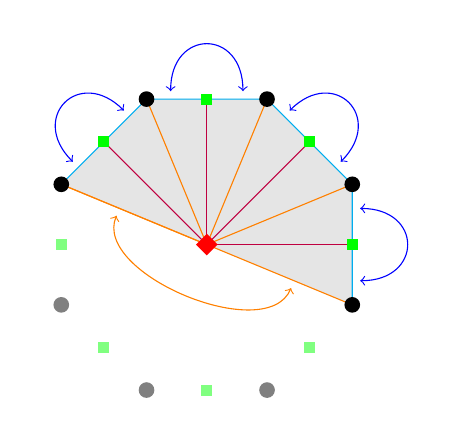
\begin{tikzpicture}[scale=2]
\coordinate (C) at (0,0);

\coordinate (A0) at (45/2:1cm);
\coordinate (A1) at (135/2:1cm);
\coordinate (A2) at (225/2:1cm);
\coordinate (A3) at (315/2:1cm);
\coordinate (A4) at (405/2:1cm);
\coordinate (A5) at (495/2:1cm);
\coordinate (A6) at (585/2:1cm);
\coordinate (A7) at (675/2:1cm);

\coordinate (B0) at (barycentric cs:A7=1,A0=1);
\coordinate (B1) at (barycentric cs:A0=1,A1=1);
\coordinate (B2) at (barycentric cs:A1=1,A2=1);
\coordinate (B3) at (barycentric cs:A2=1,A3=1);
\coordinate (B4) at (barycentric cs:A3=1,A4=1);
\coordinate (B5) at (barycentric cs:A4=1,A5=1);
\coordinate (B6) at (barycentric cs:A5=1,A6=1);
\coordinate (B7) at (barycentric cs:A6=1,A7=1);

\fill[gray!20] (A7) -- (A0) -- (A1) -- (A2) -- (A3) -- (A7);

\draw[purple] (C) -- (B0);
\draw[purple] (C) -- (B1);
\draw[purple] (C) -- (B2);
\draw[purple] (C) -- (B3);

\draw[orange] (A7) -- (A3);
\draw[orange] (C) -- (A0);
\draw[orange] (C) -- (A1);
\draw[orange] (C) -- (A2);
\draw[orange] (C) -- (A3);

\draw[cyan] (A7) -- (A0) -- (A1) -- (A2) -- (A3);

\draw[blue,<->]
 (0:.05cm) +(barycentric cs:A7=4,A0=1)
 .. controls +(0:.4cm) and +(0:.4cm) ..
 +(barycentric cs:A7=1,A0=4);
\draw[blue,<->]
 (45:.05cm) +(barycentric cs:A0=4,A1=1)
 .. controls +(45:.4cm) and +(45:.4cm) ..
 +(barycentric cs:A0=1,A1=4);
\draw[blue,<->]
 (90:.05cm) +(barycentric cs:A1=4,A2=1)
 .. controls +(90:.4cm) and +(90:.4cm) ..
 +(barycentric cs:A1=1,A2=4);
\draw[blue,<->]
 (135:.05cm) +(barycentric cs:A2=4,A3=1)
 .. controls +(135:.4cm) and +(135:.4cm) ..
 +(barycentric cs:A2=1,A3=4);

\draw[orange,<->]
 (-225/2:.05cm) +(barycentric cs:A7=4,A3=1)
 .. controls +(-225/2:.4cm) and +(-225/2:.4cm) ..
 +(barycentric cs:A7=1,A3=4);


\node[diamond,fill=red,inner sep=2pt] at (C) {};

\foreach \x in {0,1,...,3}
{
  \node[circle,fill=black,inner sep=2pt] at (A\x) {};
  \node[rectangle,fill=green,inner sep=2pt] at (B\x) {};
}
\node[circle,fill=black,inner sep=2pt] at (A7) {};
\foreach \x in {4,5,6}
{
  \node[circle,fill=black!50,inner sep=2pt] at (A\x) {};
  \node[rectangle,fill=green!50,inner sep=2pt] at (B\x) {};
}
\node[rectangle,fill=green!50,inner sep=2pt] at (B7) {};
\end{tikzpicture}%
\end{document}
